\section{Gr\ae{}nser}
\begin{frame}{Gr\ae{}nser}
\begin{itemize}
	\item Den \o{}vre gr\ae{}nse	
	\begin{itemize}
		\item 22
		\item Rokicki's set solver
	\end{itemize}
	\item Den nedre gr\ae{}nse	
	\begin{itemize}
		\item 20
		\item Super flip
	\end{itemize}
	\item Fremtiden
\end{itemize}
\end{frame}

\subsection{Den \O{}vre Gr\ae{}nse}
\begin{frame}{Den \O{}vre Gr\ae{}nse}
\only<1>{
\begin{figure}
	\centering
		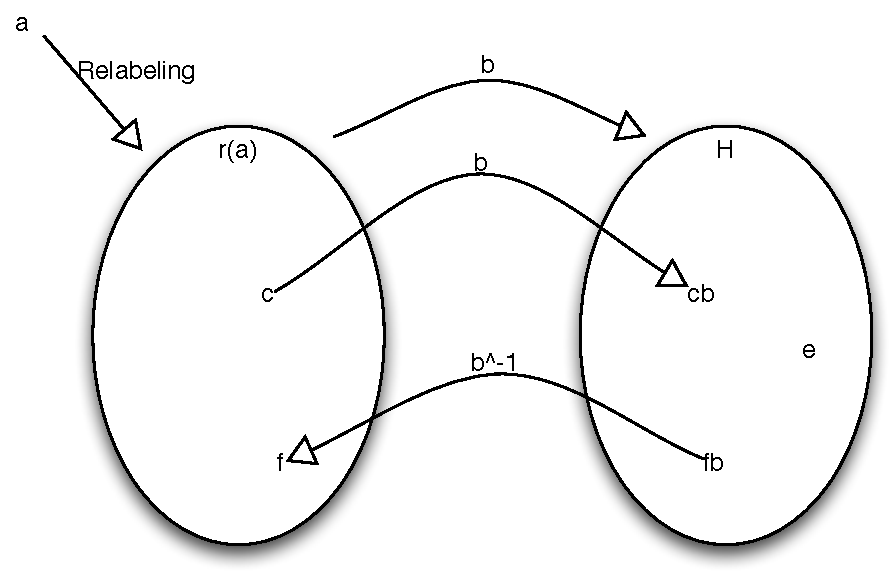
\includegraphics[width=0.9\textwidth]{input/pics/Rokiki1.pdf}
	\label{fig:Rokiki1}
\end{figure}}

\only<2>{
\begin{figure}
	\centering
		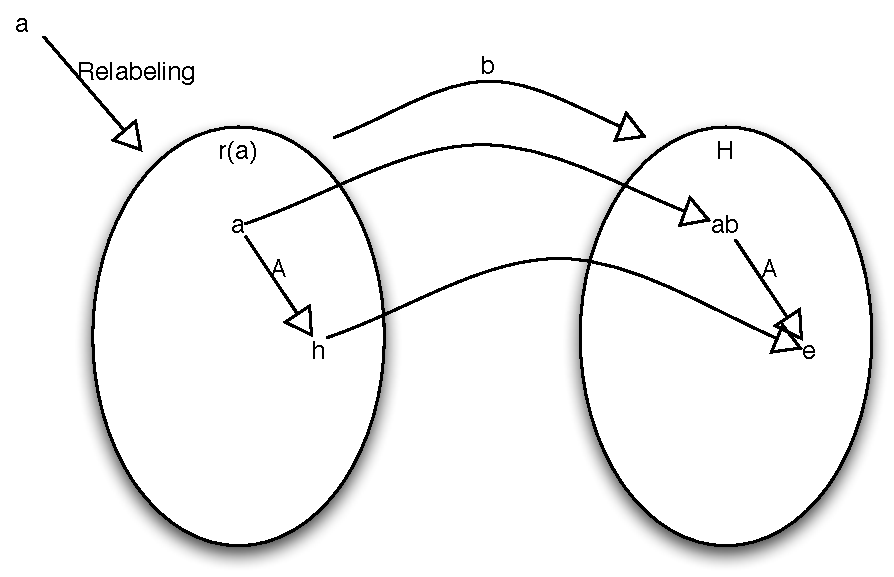
\includegraphics[width=0.9\textwidth]{input/pics/Rokiki2.pdf}
	\label{fig:Rokiki2}
\end{figure}}

\only<3>{
\begin{figure}
	\centering
		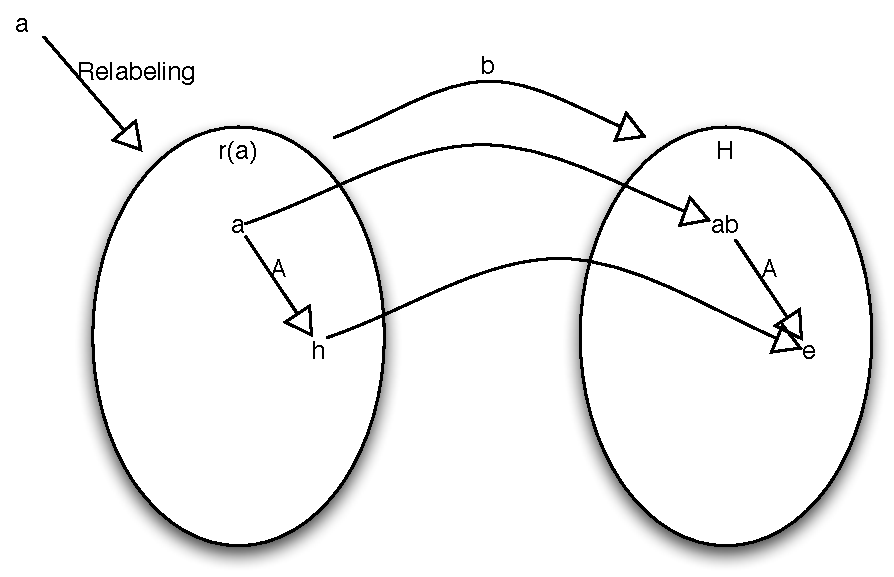
\includegraphics[width=0.9\textwidth]{input/pics/Rokiki3.pdf}
	\label{fig:Rokiki3}
\end{figure}}
\end{frame}

\subsection{Den Nedre Gr\ae{}nse}
\begin{frame}{Den Nedre Gr\ae{}nse}
\begin{figure}
	\centering
		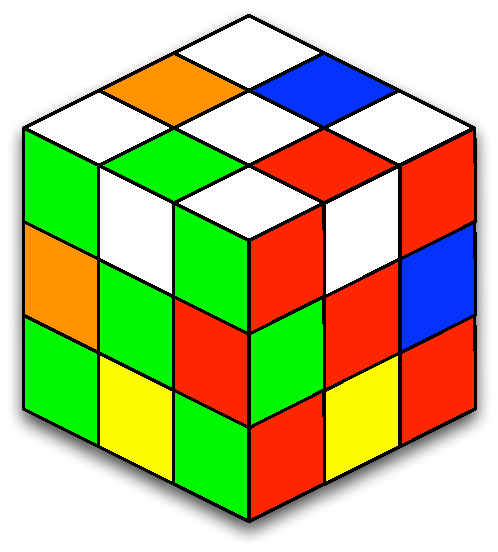
\includegraphics[width=0.75\textwidth]{input/pics/superflip.pdf}
	\label{fig:superflip}
\end{figure}

\end{frame}

\subsection{Fremtiden}
\begin{frame}{Fremtiden}
\begin{figure}
	\centering
		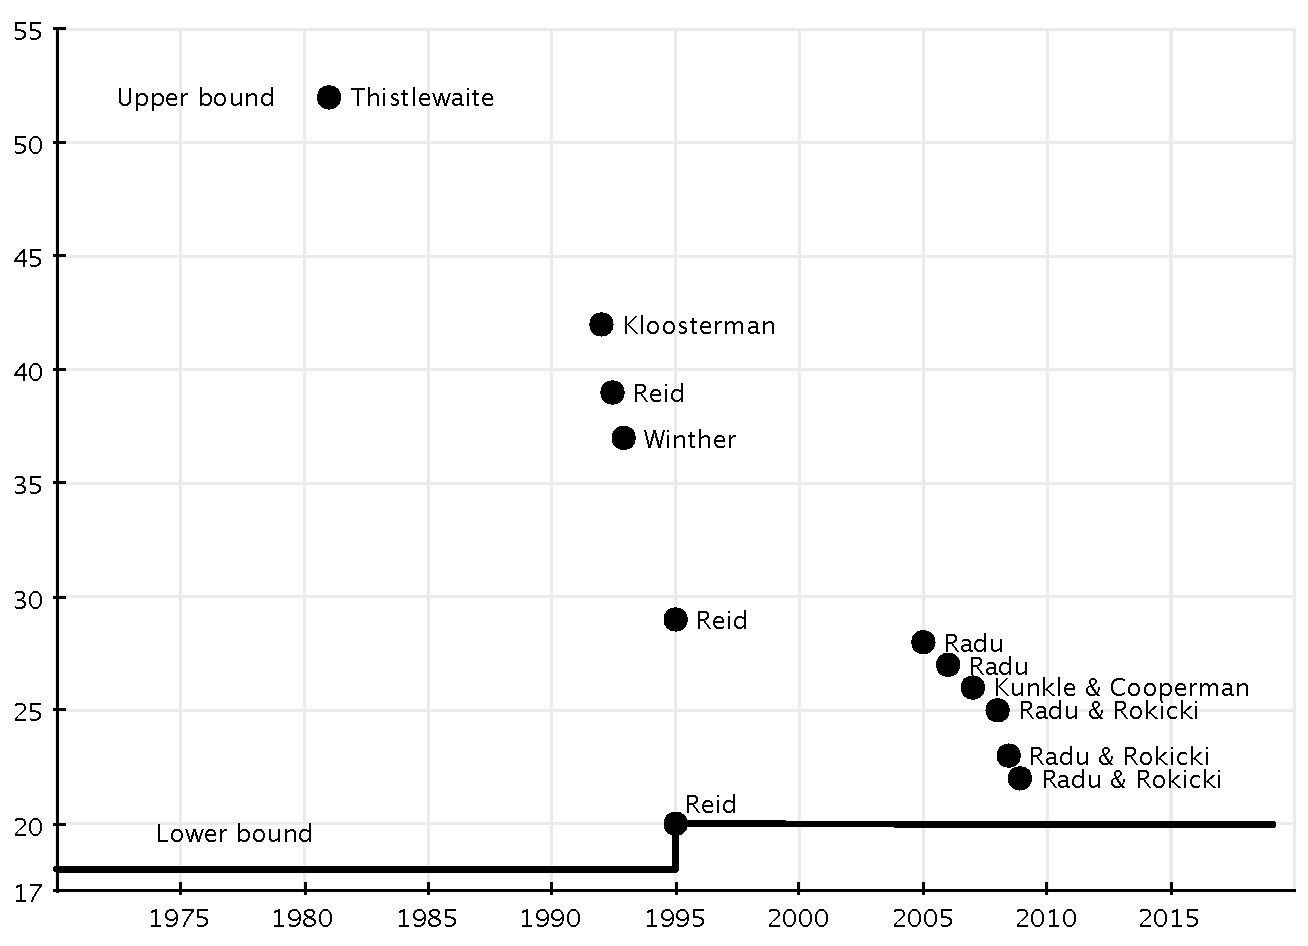
\includegraphics[width=0.9\textwidth]{input/pics/bounds2.pdf}
	%\caption{Udvikling af gr�nserne}
	\label{fig:bounds2}
\end{figure}
\end{frame}